\documentclass[11pt]{article} 

\usepackage{amsmath}
\usepackage{verbatim}
\usepackage{comment} 
\usepackage{algorithm}
\usepackage{algorithmic}
\usepackage{amsfonts}
\usepackage{amssymb}
%\usepackage{amsmath}
\usepackage{subfigure}
\usepackage{multirow}
\usepackage{flushend}
\usepackage{caption}
%\usepackage{xspace}
%\usepackage{xcolor}
%\usepackage{enumitem,url}
\usepackage{deauthor,times,graphicx}

\begin{document}
\title{Capturing Human Factors to Optimize Crowdsourced Label Acquisition through Active Learning }

\author{
Senjuti Basu Roy\\
New Jersey Institute of Technology\\
senjutib@njit.edu}


\date{}

\maketitle
\vspace{-0.2in}
\begin{abstract}
\vspace{-0.2in}
The goal of this article is to propose an {\em optimization framework by acknowledging human factors to  enable label acquisition through active learning }. In particular, we are interested to investigate tasks, such as, providing (collecting or acquiring) and validating labels, or comparing data using active learning techniques. Our basic approach is to take a set of existing {\em active learning techniques for a few well known supervised and unsupervised algorithms, but study them in the context of crowdsourcing, especially considering worker-centric optimization (i,e., human factors)}. Our innovation lies in  designing optimization functions that appropriately capture these two fundamental yet complementary facets, performing systematic investigation to understand the complexity of such optimization problems, and designing efficient solutions with theoretical guarantees.
\end{abstract}


%\newcommand{\hide}[1]{}


\section{Introduction}
% Based on this Google Doc: 
% https://docs.google.com/document/d/1e4_mH7MMYO3bad9BoknrRlWR4jOcKNOFV8UyYLU5kPA/edit

% Apple and Google recently joined forces to develop a new privacy-preserving mobile contact tracing protocol that leverages the hardware in all modern phones to automate contact tracing without revealing information about their users.  
% Despite its potential, this new protocol and how it is being deployed has created tension with governments around the world who are legitimately concerned that it will hinder manual contact tracing and undermine their ability to manage the spread of the virus. 

% Apple and Google have adopted a decentralized approach arising out of academic research that seeks to preserve privacy.   
% All contact identification and risk analysis is done locally on individuals phones without revealing where the contact event took place or the identity of the infected individual.   
% The protocol does not use location information and instead relies on the low-power Bluetooth hardware present on all modern phones.  
% The protocol is entirely opt-in and the only information that is ever shared with public authorities are non-identifying cryptographic keys provided by the COVID-positive individuals.

% However, many governments and public health authorities are advocating for a centralized approach where they maintain a record of the locations and interactions between individuals and can compute potential exposures from confirmed individuals and notify people directly.  Furthermore, location information allows them to better understand where and how the disease is spreading, so they can take preventative measures. While the utility of centralized and attributable contact tracing is critical to re-opening the world’s economy, it also raises profound concerns for civil liberties and personal privacy.

% The tech giants have taken an unprecedented position -- essentially dictating public policy by prohibiting contact tracing apps that rely on the new protocols from collecting location information.  Further, they are restricting access to the new contact tracing APIs to national governments and permitting only one app per country or region.  This decision circumvents the local governments, tribal organizations, and community health services that are often most aware of the needs of their communities and the nexus of existing manual contact tracing efforts.  Meanwhile, governments who have attempted to launch their own contact tracing apps have failed due to restrictions imposed by the Apple and Google operating systems.

% Path Forward: Both of these positions have rational basis, significant merits, and faults.  Generally, all would agree that we want to both preserve civil liberties and improve the efficacy of public health processes for detecting, containing, and mitigating the spread of the virus.  Our phones and our cooperation can be an essential part of the solution. It is well established that the Apple and Google approach is only effective if a large fraction of the population participates, but without very clear protection of personal privacy, the needed level of participation will not occur in a free society.  

% Surprisingly, with two simple measures, we can return authority to local communities without fragmenting contact tracing efforts, support manual contact tracing efforts, and provide visibility into the spread of disease all within the proposed privacy-preserving decentralized approach outlined by Apple and Google. In the rest of this article, we outline these two simple measures and how they both improve contact tracing while also preserving individual privacy.



%%%%%%%%%%%%%%%%%%%%
% START LIGHTHOUSE %
%%%%%%%%%%%%%%%%%%%%

% Governments around the world have become increasingly frustrated with tech giants dictating public health policy. The software created by Apple and Google enables individuals to track their own potential exposure through collated exposure notifications. However, the same software prohibits location tracking, denying key information needed by public health officials for robust contract tracing. This information is needed to treat and isolate COVID-19 positive people, identify transmission hotspots, and protect against continued spread of infection.


Apple and Google have adopted a decentralized approach to mobile contact tracing that prioritizes individual privacy~\cite{agen}. Under the Apple-Google Exposure Notification (AGEN) protocol (see Fig.~\ref{fig:contact_tracing}), individual phones determine if the user has been exposed, without revealing \emph{the identity of the infected individual} and \emph{where the contact event took place}
The AGEN protocol is related to contemporaneously proposed protocols including PACT and DP-3T~\cite{pact,dp3t}.
Like these other protocols, the AGEN protocol does not use location information. 
Instead, it relies on the Bluetooth radios present on all modern phones to detect proximity with others. 
Beyond not collecting Protected Health Information (PHI), the decentralized approach retains the non-PHI on the phone, allowing individuals to determine risk locally on their device.

\begin{figure}[t]
    \centering
    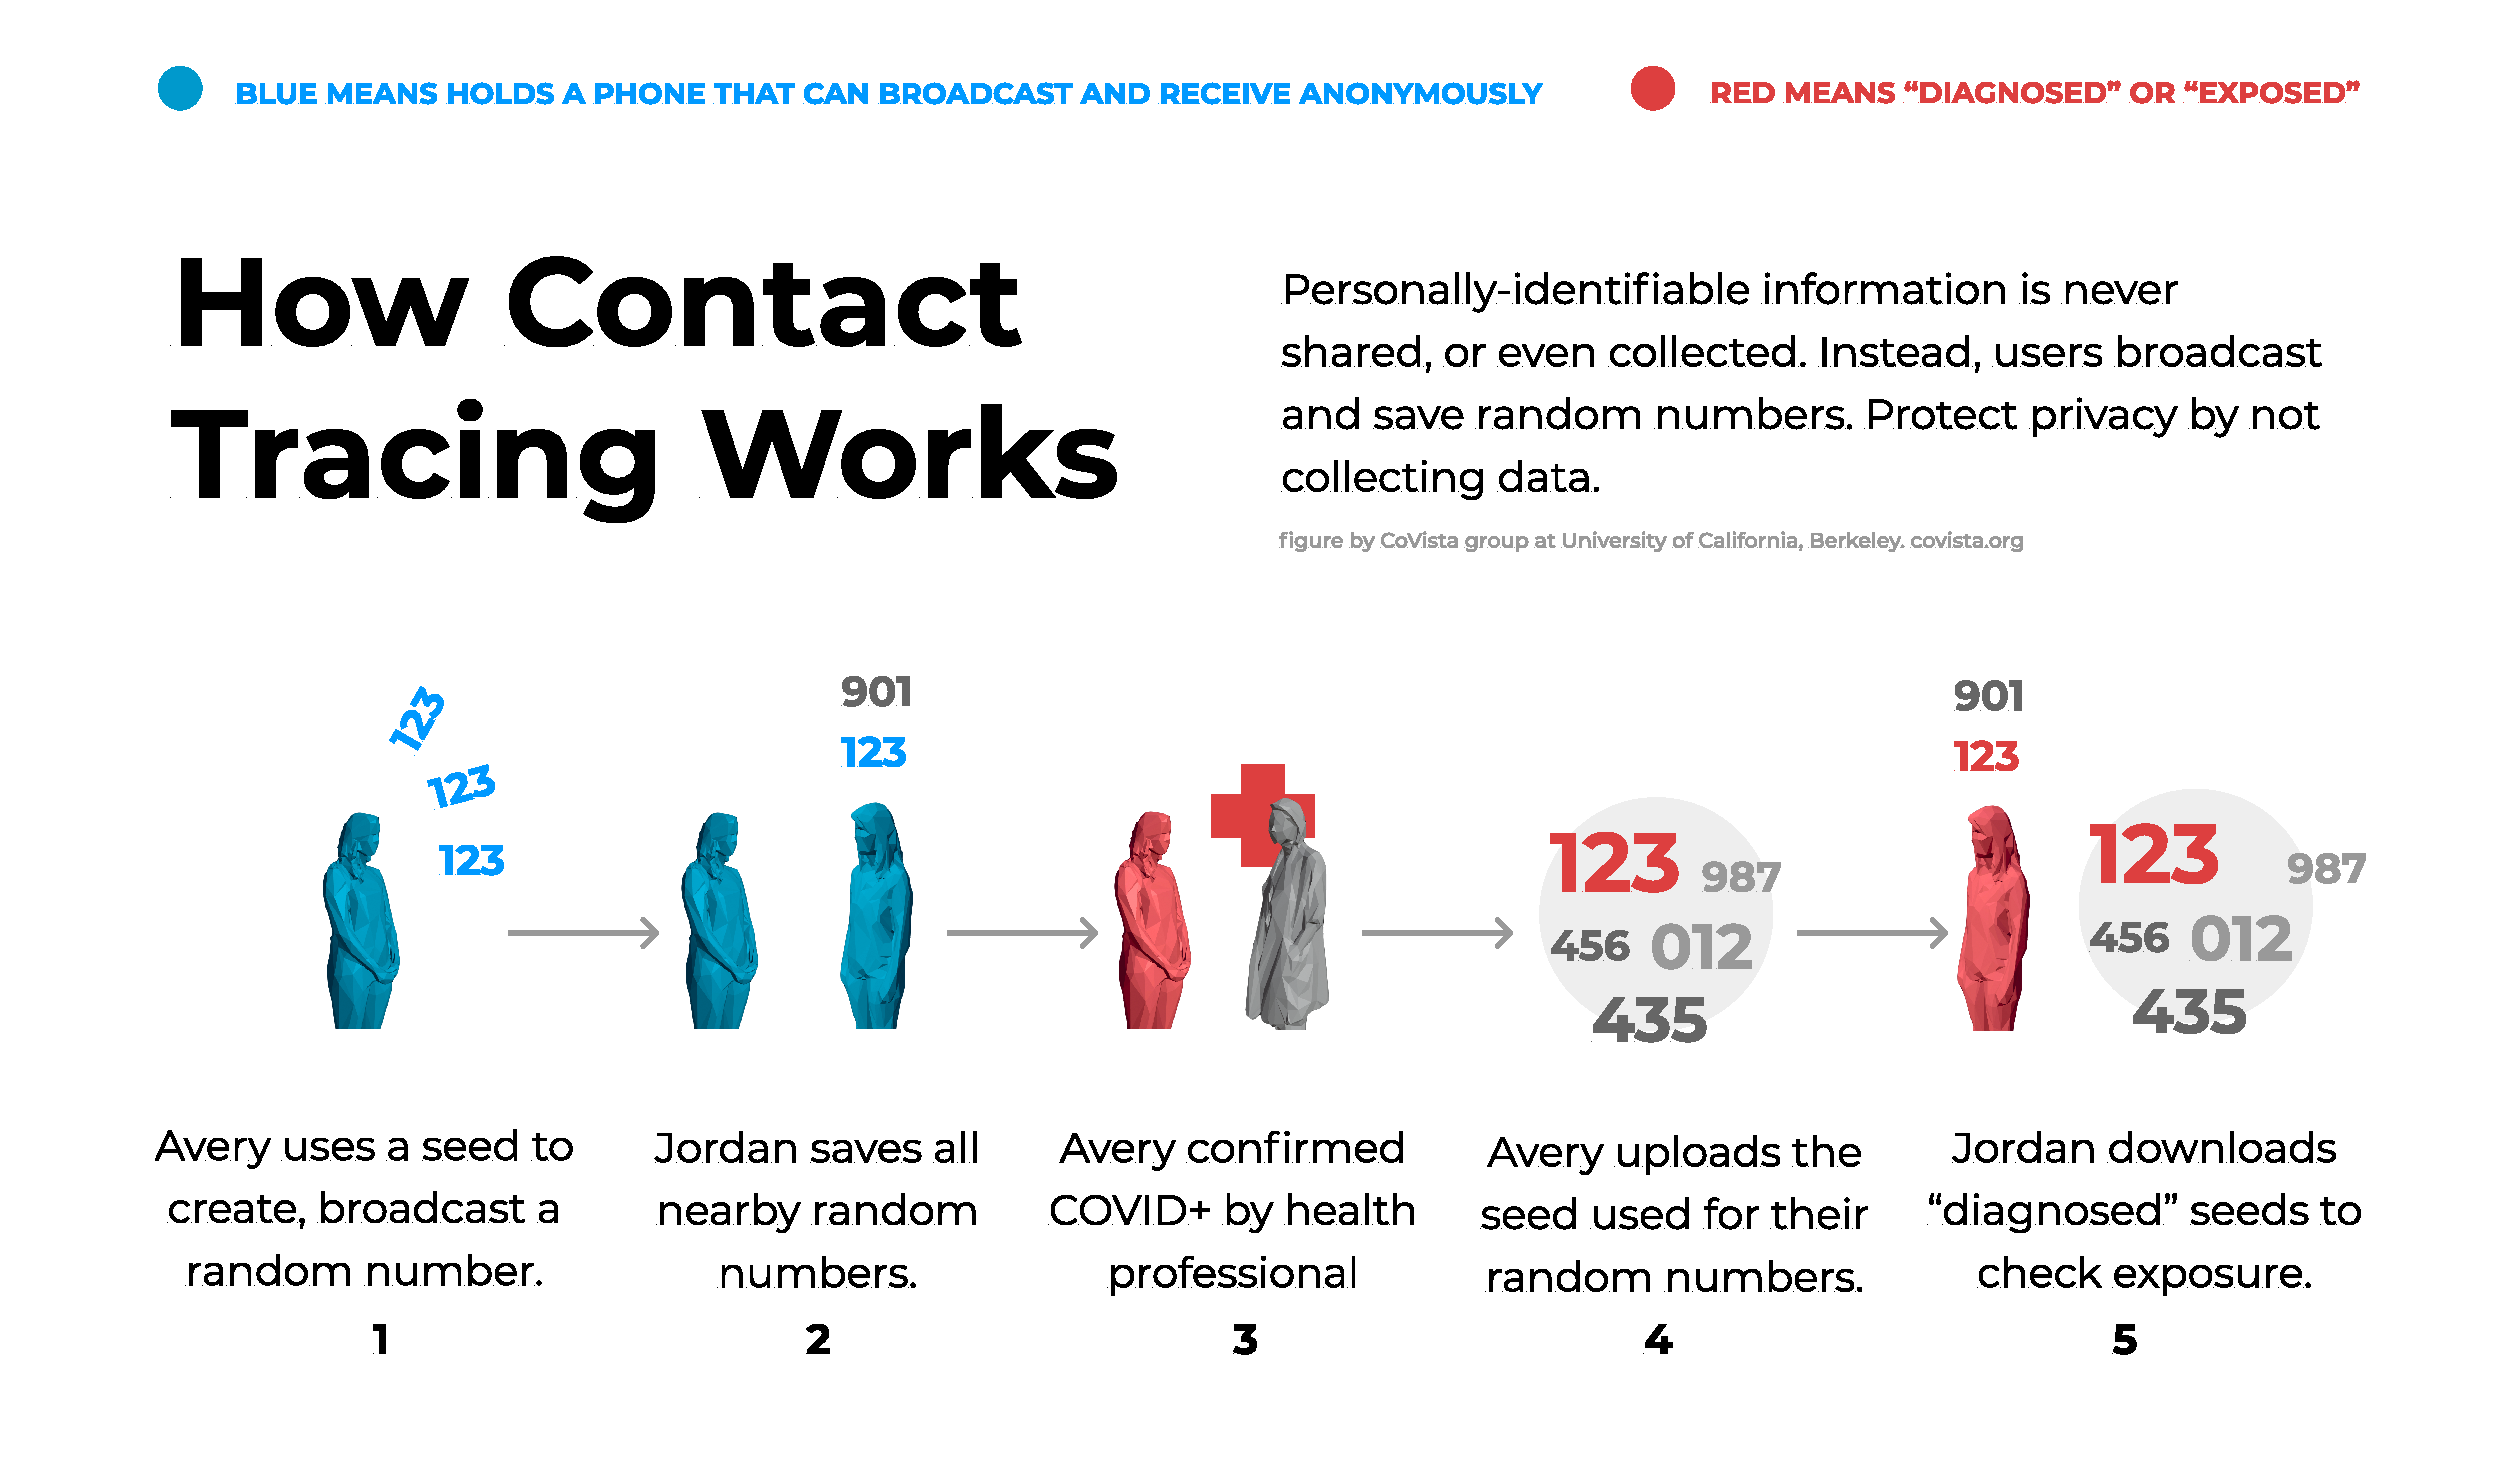
\includegraphics[width=0.8\textwidth]{figs/how_contact_tracing_works.pdf}
    \caption{Apple-Google Exposure Notification (AGEN) Protocol Overview.}
    \label{fig:contact_tracing}
\end{figure}

Governments and public health authorities want to understand where and how the disease is spreading, so they can take preventative measures.  
They also want to be able to use mobile contact tracing to augment existing manual contact tracing efforts.
With these goals in mind, governments advocate for a centralized approach, whether national or regional, where they maintain records of each person’s locations and interactions. 
This allows governments to determine exposures and notify people directly, as timeliness reduces spread. 
While centralized contact tracing may offer utility critical to re-opening the world’s economy, it raises profound concerns for civil liberties and personal privacy.
Government efforts that avoid reliance on the industrial Exposure Notification offerings have run into a host of failings, including reliability, power drain, interoperability, and participation.

Apple and Google have taken an unprecedented position -- essentially dictating public policy, not just by requiring the decentralized approach, but also by prohibiting contact tracing apps from collecting location information.
Further, they are restricting access to the new contact tracing APIs to national governments and permitting only one app per country or region. 
This decision circumvents the local governments, tribal organizations, and community health services that are often most aware of existing manual contact tracing efforts and the needs of their communities.  
Meanwhile, government contact tracing apps have failed due to restrictions imposed by AGEN.

In this article, we present two simple measures that enable the AGEN protocol to support manual contact tracing efforts, provide visibility into the spread of disease, and return authority to local communities all while preserving privacy within the Apple and Google framework. 
\begin{enumerate}
\item \textbf{Treat places as people.} Endow public places with the same privacy-preserving technology used to monitor exposure for individuals.
\item  \textbf{Nation-scale data, not apps and processes.} Build a common backend for the AGEN protocol that spans apps and governmental boundaries.
\end{enumerate}

In the rest of this article, we describe these two simple measures and how they both improve contact tracing while also preserving individual privacy.

\subsection*{Lighthouse: Treat Places as People}
\begin{figure}[h]
    \centering
    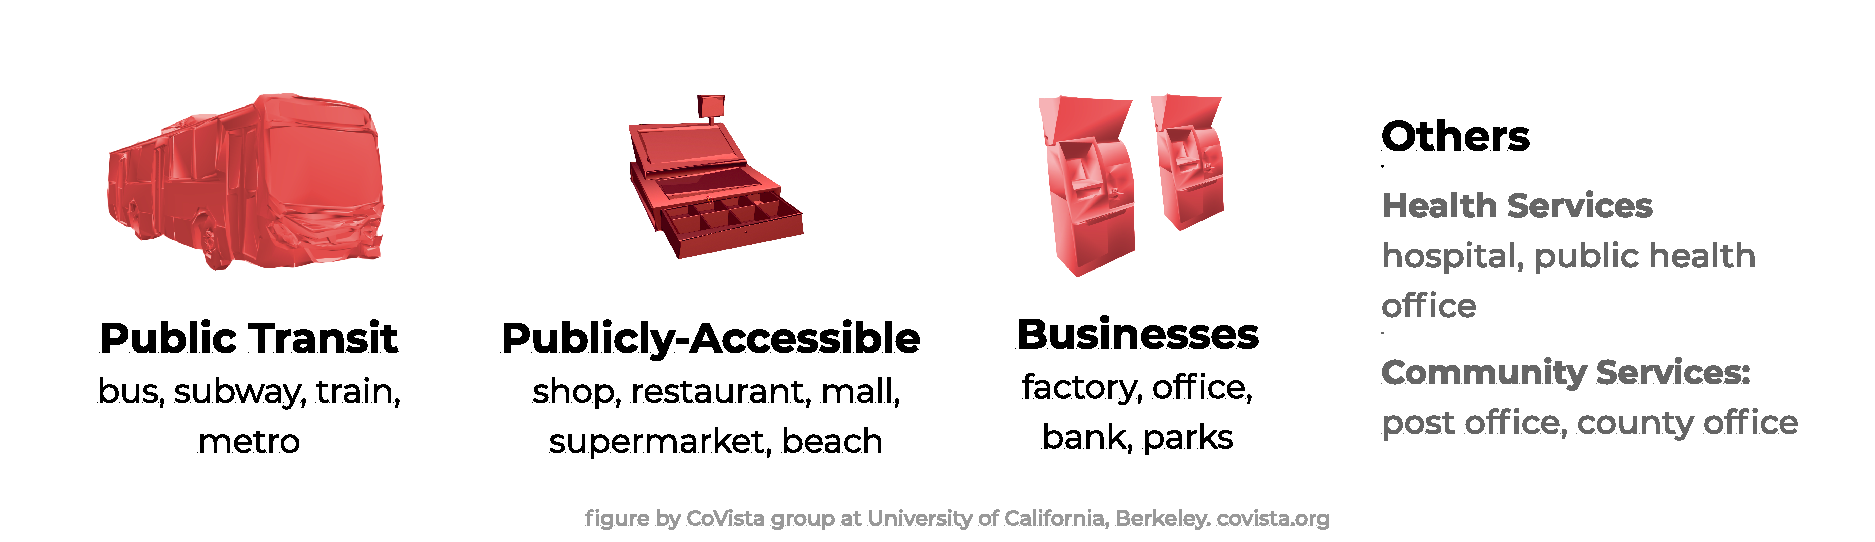
\includegraphics[width=\textwidth]{figs/places.pdf}
    \caption{Lighthouses can extend the AGEN protocol to physical places}
    \label{fig:placesExamples}
\end{figure}

If we treat public places as people, we can use the AGEN protocol to (a) understand COVID-19 exposures across space, (b) integrate with manual contact tracing, and (c) do so with the same privacy-sensitive protocol. To treat places as people in AGEN, simply attach mobile phones or specialized low-cost beacons to publicly accessible places (e.g., county services, stores, buses).  
Like a lighthouse, these devices help communicate risk associated with places.  
Well-positioned, they can offer robust proximity detection, can detect their exposure, and can convey aspects the risk that represents.

By choosing to share their locally computed exposure risk with public health authorities through the AGEN protocol, owners of publicly-accessible places can aid in mitigating virus spread. 
Alternatively, if a place is identified through traditional, manual contact tracing, the place can still anonymously participate in the AGEN protocol, notifying others without revealing where they were exposed. 
Treating places as people empowers stewards of public spaces to collaborate with public health authorities to help mitigate the spread of disease without jeopardizing the privacy of patrons or the reputation of the public spaces.
This procedure can facilitate detection of exposure from a non-participating individual while improving anonymity over manual contact tracing methods.  Going even further, such places could provide other means of beaconing that do not involve smartphones, such as QR code displays, codes on receipts and so on.

\subsection*{COVID Commons: A Nation-scale Data Backend}

Rather than “one app per nation,” a better solution would be to provide a common privacy-preserving data exchange across apps and administrative boundaries — a Commons.  This would allow societal structures and innovation, rather than corporate policy, to determine how the app ecosystem should evolve.  It is very likely that participation will be greatest if the apps are available through local organizations (e.g., tribal organization, university campus) that individuals trust.   A common privacy-preserving data exchange is already compatible with the AGEN protocol.

\begin{figure}[h]
    \centering
    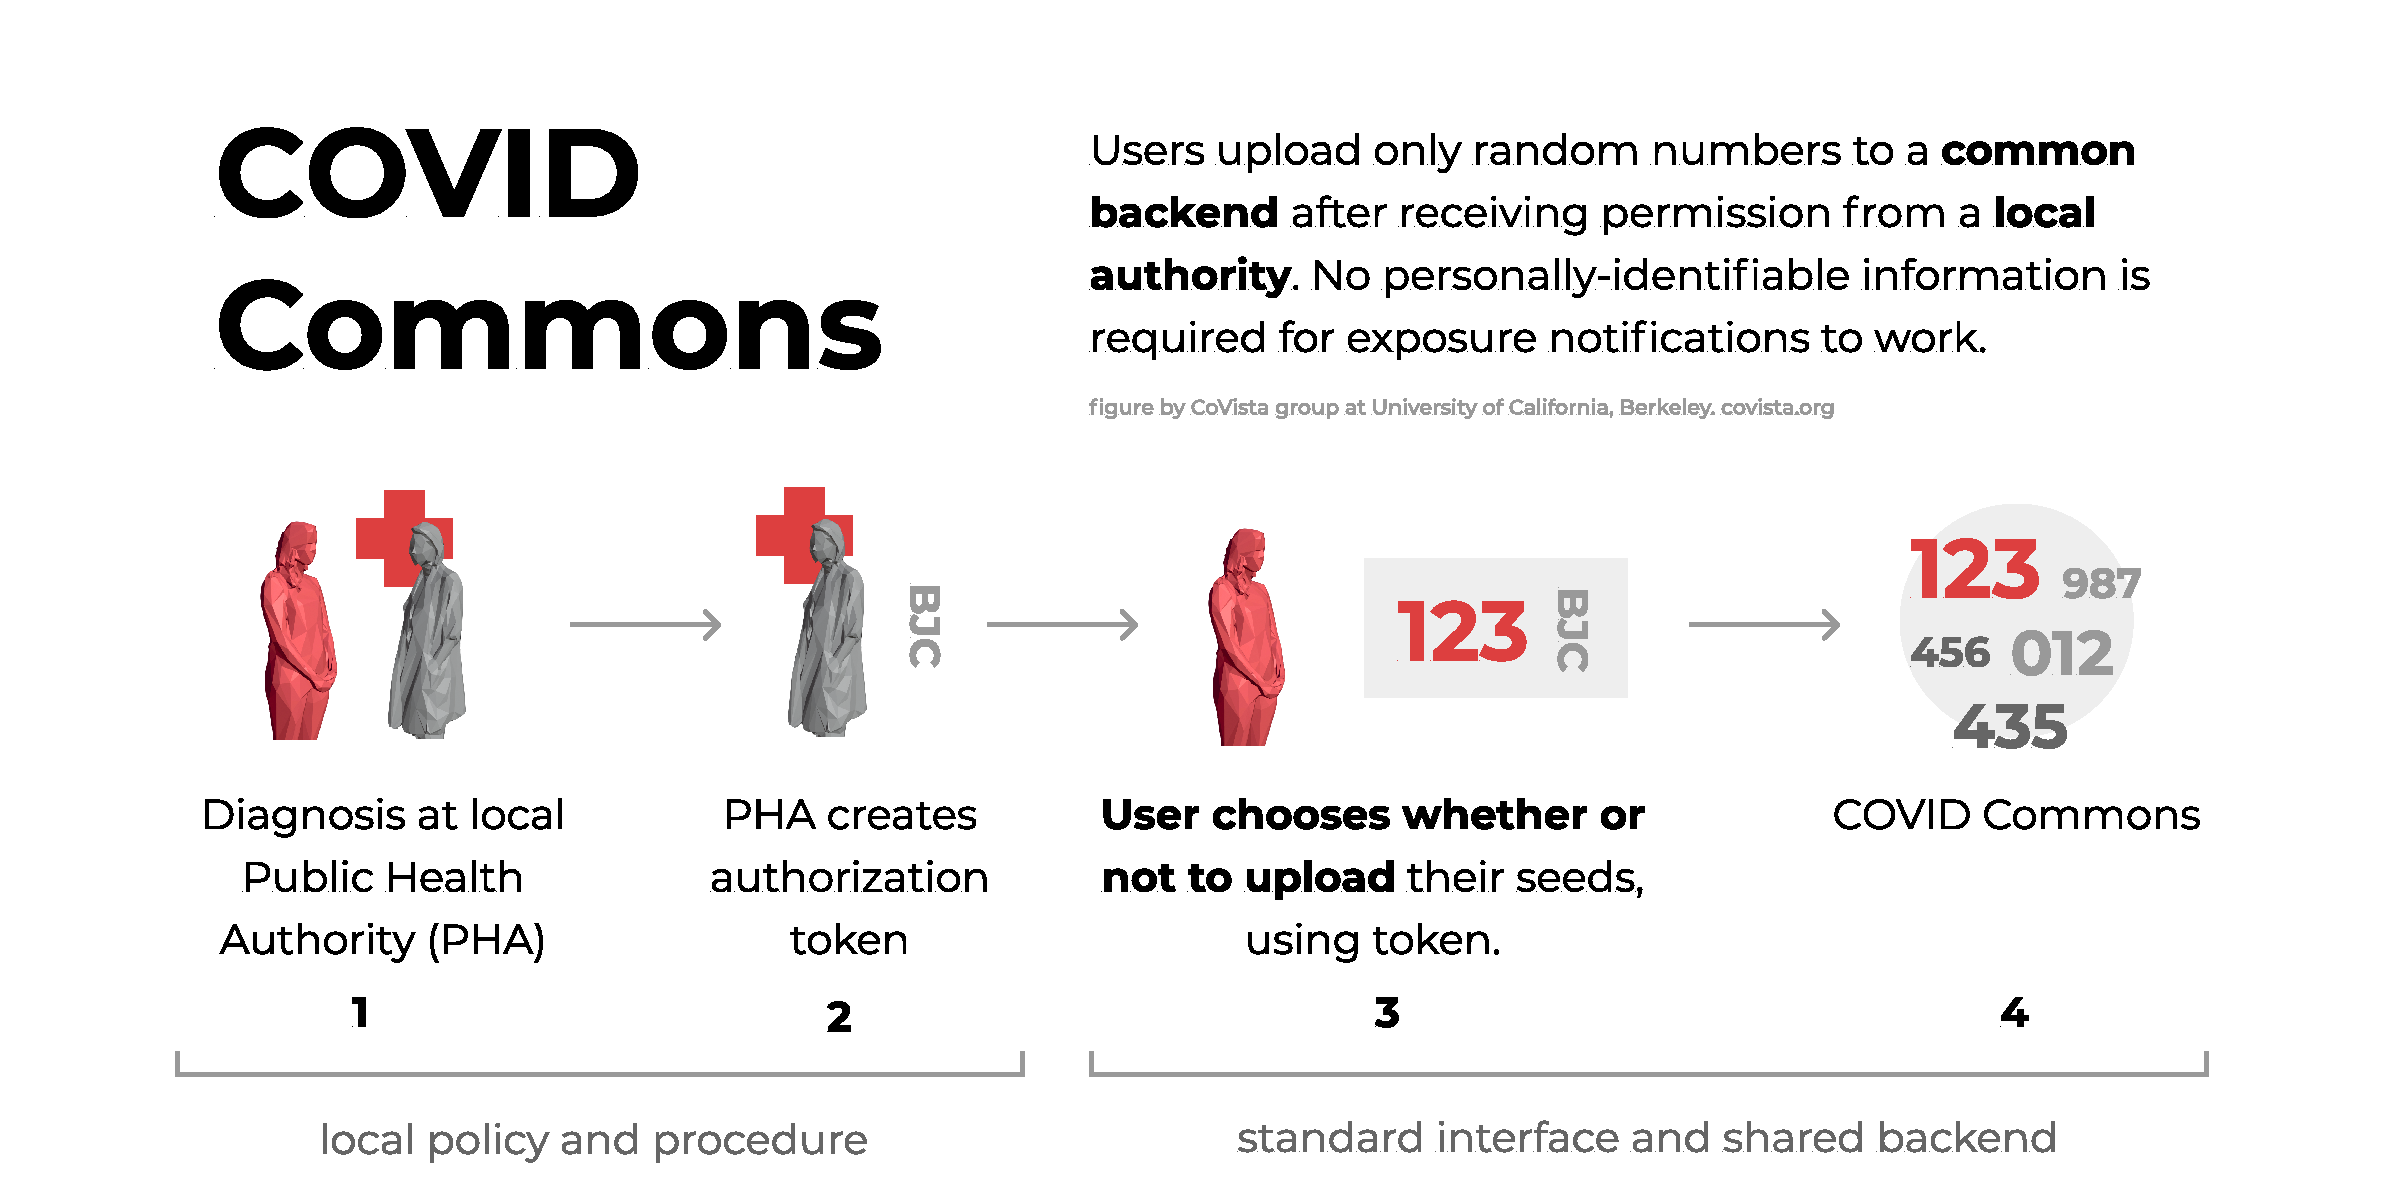
\includegraphics[width=\textwidth]{figs/covid_commons.pdf}
    \caption{Covid Commons exposure notification process.}
    \label{fig:commoms}
\end{figure}

When an individual tests positive and they engage in a conventional contact tracing interview with a public health professional. The professional obtains an authorization so the individual, on an opt-in basis, can share their anonymous exposure information.  Public health professionals serve to protect the integrity of the information in the Commons without exposing any patient data or medical data. \shankari{individual obtains authorization from professional. "an authorization"? is something like "token" missing?}

Their actions are quite similar to publishing counts of cases, statistics and demographic information, as is done today.  The Commons might be hosted by governmental or NGO structures, based on national or regional policy.  A diverse and innovative app ecosystem can grow to meet the needs of individuals and agencies.

In the remainder of this article we describe both these technical solutions in greater detail.  
We have organized each section to be relatively self-contained.

\vspace{-0.2in}
\section{Data Model}\label{dm}
\vspace{-0.1in}
We introduce different variables and characterize human factors~\cite{hf1,motiv00,motiv0,motiv1,motiv2,motiv3,motiv4}. A crowdsourcing platform typically comprises of workers and tasks that serve as the foundation of the framework we propose. We also note that not all the variables are pertinent to every application domain (for example, citizen science applications are usually voluntary contributions). Our effort is to propose a generalization nevertheless. 

{\bf Domains/types:} A set $D=\{d_1,d_2,\ldots,d_{l}\}$  of given domains is used to describe the different types of tasks in an application. Using Example~\ref{ex1}, a particular species may construe a domain. 

{\bf Workers:} A set of $m$ human workers $\mathcal{U}=\{u_1,u_2,\ldots,u_m\}$ are available in a crowdsourcing platform.
% Each worker $u$ is described by a set of  {\em human factors}~\cite{hf1,motiv00,motiv0,motiv1,motiv2,motiv3,motiv4}, i.e., variables that are important to understand their behavior in a crowdsourcing platform.

{\bf Tasks and sub-tasks:} A task $\mathcal{T}$ is a hybrid human-machine computational task (classification for example), with a quality condition $Q^\mathcal{T}$  and an overall monetary budget $B^\mathcal{T}$ that decide its termination. Using Example~\ref{ex1}, $\mathcal{T}$ is a classification task which terminates, when $Q^\mathcal{T} = 80\%$ accuracy is achieved, or $B^\mathcal{T} =\$100$ is exhausted.

Without loss of generality, $\mathcal{T}$  comprises of a set of $n$ subtasks, i.e., $\mathcal{T} =\{t_1,t_2,\ldots,t_n\}$. These sub-tasks are of interests to us,  as workers will be involved to undertake these sub-tasks. Each sub-task can either be performed by human workers or computed (inferred) by machine algorithms. We consider {\em pool based active learning}, where a finite pool of sub-tasks exists and given.

{\em Sub-tasks:}
For single label, a sub-task is an unlabeled instance of the data that requires labeling. Considering Example~\ref{ex1}, this is analogous to confirming the presence or absence of a species in a particular geographic location. 
%To generalize, we consider similar settings as that of {\em pool-based active learning}, where a pool of unlabeled instances are available for further labeling.
For multi-label scenario, a sub-task requires multiple labels to be obtained. Using Example~\ref{ex1}, this is analogous to obtaining Kingdom, Phylum, Class, Order, etc of the insect.

{\bf Worker Response:} We assume that a worker $u$'s {\em response to a particular sub-task $t$ may be erroneous, which is used by the machine algorithm in one or more rounds of interactions}. Our framework may ask multiple workers to undertake the same task to reduce the error probability, and may decide which questions to ask in the next round to whom based on the answers obtained in the previous round.

{\bf Human Factors:} These are the variables that characterize the behavior of the workers  in a crowdsourcing platform~\cite{hf1,motiv00,motiv0,motiv1,motiv2,motiv3,motiv4}.

{\em Skill (Expertise/Accuracy):}  Worker's skill in a domain is her expertise/accuracy. Skill of a worker in a domain $d$ is quantified in a continuous $[0,1]$ scale (to allow a probabilistic  interpretation). A worker $u$ may have skills in one or more domains (e.g., different species observation accuracy). 
%Given $l$ domains, $u$'s skill is described by a $l$-dimensional vector, where $s^{u_i}$ is her skill in the $i$-th domain. 

{\em Wage:} A worker $u$ may have a fixed wage $w_u$, or may have to accept the wage a particular task offers. $u$'s may have different wage for different types of tasks.

{\em Motivation:} Motivation aims at capturing the worker's willingness to perform a task. A related work~\cite{motiv1} proposes a theoretical foundation in motivation theory in crowdsourcing platform and characterizes them in two different ways: 

{\em (a) Intrinsic motivation:} Intrinsic motivation exists if an individual works for fulfillment generated by the activity (e.g. working just for fun). Furthermore, related works~\cite{motiv1,motiv2,motiv3} have identified that intrinsic motivation emerges in the following ways: (1) skill variety (refers to the extent to which a worker can utilize multiple skills), (2) task identity (the degree to which an individual produces a whole, identifiable unit of work, versus completion of a small unit which is not an identifiable final product), (3) task significance (the degree to which the task has an influence over others), (4) autonomy (the degree to which an individual holding a job is able to schedule his or her activities), (5) feedback (the extent to which precise information about the effectiveness of performance is conveyed). 

%Hackman and Oldham~\cite{hackman1976motivation} have combined these factors mathematically and defined {\em motivating potential score (MPS)} to capture intrinsic motivation:

%\begin{equation}\label{eqn}
%\begin{aligned}
%MPS= \frac{\text{skill-variety} + \text{task-identity} + \text{task-significance}}{3}  \\
%* \text{ autonomy } * \text{ feedback}
%\end{aligned}
%\end{equation}


{\em (b) Extrinsic motivation:} Extrinsic motivation is  an instrument for achieving a certain desired outcome (e.g. making money).

%{\em Acceptance ratio:} Acceptance ratio describes the {\em probability} at which a worker actually participates in a task (notice that a worker can always decline a task).Acceptance ratio may be correlated to worker motivation.
 %Given $l$ domains, $u$'s acceptance ratio is described by a $l$-dimensional vector $A^u$. 

The challenge however is, either the values of these factors have to be explicitly given or they have to be estimated. Related works, including our own, have proposed solutions to estimate skill~\cite{skill,DBLP:conf/kdd/JoglekarGP13} by analyzing historical data. %Acceptance ratio or wage of the workers are estimated by designing surveys and asking explicit questions~\cite{roy2015task}.
Nevertheless, we are not aware of any effort that models motivational factors or design optimization involving them.

{\em Worker specific constraints:} Additionally, a worker may specify certain constraints (e.g., can not work more than $6$ hours, or travel farther than $10$ miles from her current location).

{\bf Characterizing sub-tasks considering human factors:}  It is easy to notice that the motivational factors described above are actually related to tasks (i.e, sub-tasks). 

Formally, we describe that a set $A$ of attributes or meta-data is available to characterize each sub-task $t$. They are its required skill-domain\footnote{\small for simplicity, we assume that each sub-task requires one skill, whereas, in reality, multiple skills may be needed for a sub-task. The latter assumption is trivially extensible by our framework.} $s^t$ , cost/wage $w^t$, duration $time^t$, location $location^t$, significance $sig^t$, identity $iden^t$, autonomy $auto^t$, task feedback $fb^t$. Each $t$, if performed correctly, contributes by a quantity  $q^t$ to $Q^\mathcal{T}$. These contributions are purely dictated by the active learning principles, such as how much it reduces the uncertainty.



%{\em Unlike other human factors, there does not exist any mathematical model that captures human motivation}. We therefore make an effort to mathematically model human motivation. 

 %and has a cost $b^t$. The cost of a sub-task is the money that has to be paid when it is performed by a human worker.

 







\vspace{-0.2in}
\section{Worker-Centric Optimization through Human Factors Modeling}\label{hf}
\vspace{-0.1in}
Recall Section~\ref{intro} and note that worker-centric optimization is a common theme across single and multi-labels tasks, which we first examine here.

{\bf Objectives:}
Our objective here is to explore mathematical models for worker-centric optimization in crowdsourcing platforms. Specifically, given an available pool of tasks and workers where workers perform repetitive tasks, we first obtain human factors of the workers by analyzing their past tasks and then study the problem of task assignment to enable worker-centric optimization. A recent work performs an ethnomethodological study at {\em Turker Nation}\footnote{\small http://www.turkernation.com/} and argues~\cite{martin2014being} that it is critical to enable worker-centric optimization.
Our effort here is to make a formal step towards that goal, independent of any specific system-centric optimization (i.e., the active learning principles). Therefore, such a study has a much broader applicability that goes beyond active learning. Of course, our framework will ultimately combine both system and worker-centric criteria. 

 {\bf Challenges:} While the significance of human factors is well-acknowledged in crowdsourcing, the challenge is to be able to estimate them effectively and propose appropriate models that could capture them during task assignment. Added to the fact is the dependence of the underlying crowdsourcing domain, which makes some of these factors more important than the rest (e.g., unlike AMT, there is no monetary pay-offs in citizen science activity, but skill variety is acknowledged to be critical to avoid monotony). 

%{\bf Our Prior Work:} In our recent investigation, we have studied some human-factors, such as, worker skill (accuracy), wage (pay-off), acceptance ratio of tasks, social affinity~\cite{hf1,roy2015task,DBLP:journals/corr/RahmanRTAD15} and proposed mathematical functions to include them explicitly in task assignment. We have designed medium-scale user studies~\cite{roy2015task,DBLP:journals/corr/RahmanRTAD15} in Amazon Mechanical Turk (AMT), involving hundreds of workers to learn the relationship between these factors and have observed that skill, wage, acceptance ratio - all follow normal distributions. We also have observed that a strong positive correlation exists between worker accuracy and expected wage. These studies have demonstrated empirically that task assignment considering human factors yields superior outcomes compared to the one without. In another recent work, we present how to combine task relevance (Boolean match of worker's expertise with the skill requirements of the tasks) and motivation in the task assignment process~\cite{edbt172}, albeit in a non-active learning context. Moreover, this work only considers {\em skill-variety} in formalizing motivation. In that sense, this latter work is still preliminary and does not solve the problem we propose. A recent survey paper summarizes different aspects of worker centricity in crowdsourcing platforms~\cite{amer2016toward}. 


\vspace{-0.1in}
\subsection{Proposed Directions}
\vspace{-0.1in}
First, we propose how to model and estimate human factors~\cite{hf1,motiv00,motiv0,motiv1,motiv2,motiv3,motiv4} that are pertinent to capture motivation using the variables that are described in Section~\ref{dm}. Then, we describe mathematical models that leverages these estimated human factors to explicitly assign tasks to workers. 

{\bf Estimating human factors:} We leverage the past task completion history of the workers as well as the new tasks to compute a Boolean task completion matrix $T$, where the rows are the workers and the columns are the (sub)-tasks. If a worker $u$ has completed a (sub)-task $t$ successfully in the past, the corresponding entry gets a $1$, it gets a $0$ otherwise. We assume that the factors that capture intrinsic motivation, i.e., skill variety, task identity, task significance, autonomy, feedback are independent yet latent variables. The second matrix we consider is the task factor matrix $\mathcal{F}$, where the rows are the tasks and the columns are the motivation related latent variables.  The final matrix is the user factor matrix $\mathcal{U}$ where rows are the factors and columns are the users. This matrix could be fully latent or observed.  In case it is latent, we minimize the error function, as defined below:

\begin{equation}
\sum_{i,j}(t_{ij}-\mathcal{U}_iF_j)^2+\lambda(\|\mathcal{U}\|^2+ \|\mathcal{F}\|^2)
\vspace{-0.1in}
\end{equation}

Here, $\lambda$ is the regularization parameter. The goal is to find ${\mathcal U}$ and ${\mathcal F}$ such that it minimizes the error. For any new worker and new task, the predicted task completion score is calculated by multiplying $U_i$ with $F_j$. Here, the important thing is to notice that the optimization function only minimizes the error for which ratings are present.  We apply the alternating least square approach~\cite{stigler1981gauss} to solve this problem. This is an iterative approach, where at each iteration, we fix the tasks' latent factor matrix $\mathcal{F}$ in order to solve for $\mathcal{U}$ and vice versa. We have designed a similar solution for predicting tasks to workers considering implicit workers' feedback\cite{DBLP:journals/corr/RahmanJR16}.

 
{\bf Worker-Centric Task Assignment:} The solution above only estimates the intrinsic motivational factors, but does not describe how to aggregate them together or combine with extrinsic motivation to perform worker-centric task assignment. 

Psychologists Hackman and Oldham~\cite{hackman1976motivation} have combined factors associated to intrinsic motivations defined {\em motivating potential score (MPS)} :

\begin{equation}\label{eqn}
\begin{aligned}
MPS= \frac{\text{skill-variety} + \text{task-identity} + \text{task-significance}}{3}  
 *\text{ autonomy } * \text{ feedback}
\end{aligned}
\end{equation}

Considering this aforementioned formulation, we study the worker-centric task assignment as a global optimization problem to maximize the {\em aggregated intrinsic and extrinsic motivation}. For a given set of tasks $S^{t_u}$,  $V(S^{t_u})$ represents the overall motivation for worker $u$, by combining  her extrinsic motivation  (EXTM) (recall Section~\ref{dm} that EXTM could be modeled using wage $w^t$) and intrinsic motivation, i.e, {\em motivating potential score (MPS)}(refer to Equation~\ref{eqn})~\cite{hackman1976motivation}. In our initial effort, we combine them linearly, as that allows us to design efficient algorithms. Assigning a set of tasks per worker is reasonable as well as desirable from worker's perspective, because workers in a typical crowdsourcing platform intend to undertake multiple tasks as opposed to a single task. Workers may also have constraints, such as,  not spend more than $X^u$ hours, 
or the aggregated wage must at least be $b^u$ dollars. 
 
Technically, we want to assign tasks to the workers {\em to maximize the aggregated motivation, such that the assignment satisfies each worker-specific constraints}. One such optimization function is described in Equation~\ref{eqn:eq3} (Recall Section~\ref{dm} where $time^t$ and $w^t$ are the duration and wage of sub-task $t$, respectively).

\begin{equation}\label{eqn:eq3}
 \text{ Maximize }  \sum_{u \in \mathcal{U}} [V(S^{t_u}) =  EXTM(S^{t_u}) + MPS(S^{t_u})]
\end{equation}
\vspace{-0.2in}
\begin{align*}
 V(S^{t_u}) =
\begin{cases} 
 \\ \text{ if } \sum_{t \in S^{t_u}} time^t \leq X^u \text{ and } \sum_{t \in S^{t_u}} w^t \geq b^u \\
0 \text{\qquad otherwise} 
\end{cases}
\vspace{-0.1in}
\end{align*} 


%Recall that a task $t$ is associated with a set $A$ of attributes, whose values, we assume are provided by the domain experts and are available at our disposal. Formally, for each task, we know the required skill domain $s^t$, duration $time^t$, significance $sig^t$, identity $iden^t$, autonomy $auto^t$, feedback $fb^t$, and wage $w^t$.

As a simple example, given two tasks $i$ and $j$, we can add the individual significance $sig^i+sig^j$, identity $iden^i+iden^j$, autonomy $auto^i+auto^j$, or feedback $fb^i+fb^j$. Similarly, the  wage of two tasks could also be added and normalized to compute EXTM. 
Alternative problem formulation is explored below.
%However, in order to compute MPS,  we still need to model and quantify the {\em skill variety} of a given set of tasks. 

%{\em Modeling Skill-variety:} We intend to study two different ways to capture skill variety. 

%(1) Set based modeling: Simple set based measures, such as, {\em Jaccard Distance}~\cite{baeza1999modern} can  be used to quantify {\em skill variety} between a given set of tasks. As an example, given $2$ tasks $t_1,t_2$ from citizen science, if $s^{t_1}=\text{humming bird}$, $s^{t_2}=owl$, skill variety $skill-variety(t_1,t_2)=1$. 

%In some application, it is reasonable to assume that an {\em intrinsic diversity ordering}~\cite{vee2008efficient} between the task attributes are available which can potentially be used to quantify skill-variety. For example, two sub-tasks associated with the same location that require to observe two different species may require more skill variety than two other sub-tasks that require observing the same species but from two different locations. We formalize this as, $\text{skill-domain} \prec \text{location}$. If such a diversity ordering is available from the domain experts, we model skill-variety considering diversity ordering~\cite{vee2008efficient}.

%(2) Order based modeling: An interesting alternative of the set based skill-variety computation  is to design an {\em ordering based}~\cite{DBLP:conf/icde/RoyDAY11,cao2012keyword} solution, where a {\em chain} of sub-tasks will be designed for a worker. Using Example~\ref{ex1}, this would mean creating an ordering $\mathcal{R}$ of the tasks for each worker where the skill-variety is ideally very high. Unlike set based approaches, here, skill-variety of a given set of sub-tasks will be computed considering each $k$ adjacent sub-tasks in the designed chain ($k=2$ means pair-wise adjacent tasks). As a simple example, if $3$ sub-tasks $t_2 \rightarrow t_1 \rightarrow t_3$ are designed for a worker, for $k=2$,  $skill-variety(t_2 \rightarrow t_1 \rightarrow t_3)= Jaccard(s^{t_2},s^{t_1})+ Jaccard(s^{t_1},s^{t_3})$.  %This modeling could also be extended when diversity based ordering between the attributes are available.


%The directions described above give rise a number of interesting computation problems.

%MPS formula requires us to quantify {\em skill variety} for a given set of tasks. We note that modeling skill variety leads to interesting research problems. Additionally, how to solve the objective function described above efficiently remains to be a challenging problem.
\vspace{-0.1in}
\subsection{Open Problems}
\vspace{-0.1in}
 {\bf  Solving the optimization problem:}
How to design an effective solution to maximize worker motivation based on the aforementioned objective function formulation is challenging. %The problem becomes even more complex when skill-variety is modeled as a chain. Even when set based modeling is considered, 
We observe that the proposed optimization problem is NP-hard~\cite{garey1979computers}, using a reduction from the assignment problems~\cite{roy2015task}. In a recent work, we have modeled motivation using {\em only skill-variety} and we have proved that the problem is NP-hard using a reduction from the Maximum Quadratic Assignment Problem~\cite{arkin2001approximating}. For our problem, we note that an integer programming based solution is simply not scalable. We will explore greedy heuristic strategies that are effective and efficient. For example, we will assign tasks to the workers greedily based on the marginal gain~\cite{roy2015task}. 
%if the set-based formulation admits {\em sub-modularity}~\cite{lovasz1983submodular}, as {\em skill-variety} exhibits {\em diminishing return properties}, and other motivational elements simply increase as more tasks are added. If this property is indeed satisfied, we will be able to design greedy approximation algorithms~\cite{nemhauser1978analysis} with theoretical guarantees. For the ordering based model, we will explore orienteering like solutions~\cite{chao1996fast} to design efficient greedy heuristic algorithms.

\noindent {\bf  Complex modeling for estimating intrinsic motivation \& task assignment:} In our preliminary direction, we have assumed that variables associated with intrinsic motivations are independent and could be combined as suggested by Hackman and Oldham~\cite{hackman1976motivation}, or intrinsic and extrinsic motivation could be combined linearly. In reality, that may not be the case. In this open problem, we will study the feasibility of a probabilistic model~\cite{zhao2012bayesian}, namely a {\em hierarchical Bayesian framework}~\cite{liu2014framework} for this problem. If the worker is completely new in the platform, we will bootstrap to collect a small set of evidence. We will consider each of the variables associated with worker motivation as a random variable and present a model using hierarchical Bayesian Networks~\cite{jensen1996introduction} by encoding a joint distribution of these variables over a multi-dimensional space.  This model will first establish the relationship among the intrinsic motivational variables themselves and then between intrinsic and extrinsic motivation to capture a workers' ``preference'' to a given task. We will apply Constraint Based, Score-Based, and Hybrid methods to learn the structure of the network~\cite{tsamardinos2006max}. We will leverage {\em Bayesian Parameter Estimation as well as Maximum Likelihood Estimation techniques} to learn the parameters of the constructed network. For efficient parameter estimation considering this complex joint distribution, we will use Gibbs sampling~\cite{carter1994gibbs}. 

%As outlined in the aforementioned open problem, if we are successful to model the motivational variables using a graphical model through probabilistic modeling, we shall extend that model to a hierarchical Bayesian Network with constraints that 

%In our preliminary work, we have assumed that variables associated with intrinsic motivation are combined as suggested by Hackman and Oldham. Moreover, we have aggregated intrinsic and extrinsic motivation linearly, as described in Equation~\ref{eqn:eq3}. In this open problem, we will explore alternative modeling. 






\vspace{-0.2in}
\subsection{Optimized Single-Label Acquisition Involving Crowd}\label{label}
\vspace{-0.1in}
We now investigate our proposed optimization framework for single-label acquisition. This problem is examined by augmenting active learning principles with worker-centric optimization (refer to Section~\ref{hf}).

{\bf Objectives:} We are assuming a setting where single-label acquisition is difficult, expensive, and time consuming (such as, Example~\ref{ex1}). We adapt a set of popular as well as well-known active learning principles\cite{al1,qbc1,qbc2,error-reduction} that are proposed to optimize system-centric cirteria, such as, {\em minimizing uncertainty or maximizing expected error-reduction} that are known to be effective in supervised (classification) algorithms~\cite{al-svm,al-svm2,al-dtree,korner2006multi}. We augment these active learning principles with worker-centric optimization. Given a pool of unlabeled instances  (of sub-tasks) and an available set of workers, the objective is to select sub-tasks for further labeling and assign workers for annotations, such that, the assignment optimizes both system and workers. The same sub-task may be annotated  by multiple workers.

{\bf Challenges:} An oracle, who knows the ground truth, no longer exists in crowdsourcing; instead, multiple workers, with varying expertise (skill), are available. Under this settings, how to realign traditional active learning goals that are system-centric (i.e., optimizes underlying computational task) requires further investigations. How to systematically design {\em optimization function}, i.e., one that combines worker-centric optimization in traditional active learning settings~\cite{active-learning-cs1,active-learning-cs2} is the second important challenge. An equally arduous challenge is the efficiency issue which is mostly overlooked in the existing research. Finally, when to terminate further label acquisition also needs to be examined.

\vspace{-0.1in}
\subsection{ Proposed Directions}
\vspace{-0.1in}
Our overall approach is iterative, where, in each round a set of sub-tasks are selected for annotation and a set of workers are chosen. Once annotations are received, the underlying classification model is retrained. After that, either the process terminates or we repeat. It has three primary directions: (1) {\em in a given round, which sub-tasks are to be selected for annotation and assigned to which workers?} (2) {\em  how to aggregate multiple annotations to obtain the ``true'' label?} (3) {\em when to stop?}  

{\em Which sub-tasks are to be selected and assigned to which workers?} We take a set of well-known active learning techniques, such as, {\em uncertainty sampling \cite{al1}, query-by-committee \cite{qbc1,qbc2}, or expected-error reduction~\cite{error-reduction}, used in popular classification algorithms, such as, Naive Bayes~\cite{entropy}, SVM~\cite{al-svm,al-svm2}, Decision Trees~\cite{al-dtree}, or ensemble classification\cite{korner2006multi}} and study them in crowdsourcing.

When a single classifier with a binary classification task is involved and the classifier is probabilistic (such as Naive Bayes), we consider existing uncertainty sampling~\cite{al1} techniques. We use entropy~\cite{entropy} to model uncertainty to choose that sub-task for labeling whose posterior probability of being positive is closest to $0.5$. For non-probabilistic classifiers (such as SVM or Decision Tree), we explore {\em heterogeneous approach}~\cite{lewis1994heterogeneous}, in which a probabilistic classifier selects sub-tasks for training the non-probabilistic classifier. We also study existing expected-error reduction~\cite{error-reduction} techniques that select the sub-tasks to minimize the expected future error of the supervised algorithm, considering {\em log-loss or $0/1$-loss}. We study the query-by-committee\cite{qbc1,qbc2} technique, we choose that sub-task for further labeling which has the {\em highest disagreement}. 

Active learning principles  mentioned above are too {\em ideal} to be useful in a crowdsourcing platform. A simple alternative is to design a {\em staged solution}, where we first select the tasks and then the workers~\cite{active-learning-cs1}. For us, we can take the task-selection solution from~\cite{active-learning-cs1} and then plug in our worker-centric optimization (Section~\ref{hf}) to compose tasks for the workers. We, however, argue that such a staged solution is {\em sub-optimal}, simply because, tasks selected by {\em active learning} techniques may end up having a very low worker-centric optimization, resulting in poor outcome overall. We therefore propose a global optimization that combines (1) worker-centric goals (recall Equation~\ref{eqn:eq3}). (2) active learning principles considering workers with varying expertise. 

Recall Section~\ref{dm} and note that $q^t$ represents sub-task $t$'s contribution towards a given active learning goal (for example, how much $t$ reduces uncertainty or expected-error) at a given iteration. Let $S^{t_u}$ represent the sub-tasks assigned to $u$ with value 
$V(S^{t_u})$ (recall Equation~\ref{eqn:eq3}). Considering worker's skill $s^{u_t}$ as a probability, $u$'s {\em expected contribution} to $t$ is  $s^{u_t} * q^t$~\cite{clemen2007aggregating}. One possible way to combine them is as a multi-objective global optimization function where the objective is to select sub-tasks and workers that maximize a weighted linear aggregation of worker and task-centric optimization (Equation~\ref{eqn:eq2}, where $W_1,W_2$ are specific weights). While linear aggregation is not the only way, it is more likely to admit efficient solutions, where the weights are tunable by domain experts (by default, $W_1=W_2=0.5$). 


%In our initial direction, we combine them in a weighted linear fashion  considering weights by combining both worker and task-centric criteria, where the latter is modeled as a linear weighted aggregation by multiplying $q^t$ with $s^{u_t}$ ($u$'s skill/accuracy in task $t$).

\begin{equation}\label{eqn:eq2}
 \text{ Maximize } \mathcal{V} =  \sum_{u \in \mathcal{U}} [W_1 * V(S^{t_u}) +  W_2 * \sum_{t \in S^{t_u}} (s^{u_t}*q^t)]
\end{equation}

Additionally, if a task has a cost budget associated that could be assigned either as a constraint to this optimization problem, or we could use cost as another objective as part of the optimization function, akin to one of our recent works~\cite{roy2015task}. Nevertheless, we acknowledge that designing the ``ideal'' optimization model that suffices the need of every application is practically impossible. We address this in the open problems.

{\em  Aggregating multiple annotations:} Another challenge is how to combine annotations from multiple workers with varying expertise to obtain the ``true'' label. We apply weighted majority voting types of approach~\cite{ho2013adaptive}, where the weights are chosen according to the skills of the workers. We also consider iterative algorithm for this purpose. Examples of iterative techniques include EM or Expectation Maximization\cite{hung2013evaluation}. The main idea behind EM is to compute in the $E$ step the probabilities of possible answers to each task by weighting the answers of workers according to their current expertise, and then to compute in the $M$ step re-estimates of the expertise of workers based on the current probability of each answer. The two steps are iterated until convergence.  We explore Bayesian solution~\cite{clemen2007aggregating} to probabilistically obtain the true label, i.e., given workers' annotations and skill, compute $Pr(t=0)$ and $Pr(t=1)$ and choose the one which has the higher probability.

%There exists a number of complex technical open problems.
\vspace{-0.1in}
\subsection{Open Problems}\label{opp}
\vspace{-0.1in}
{\bf  Solving the optimization problem} Solving the optimization problem described above is challenging. In a very recent work, we have formalized  task assignment as a linear combination of task relevance (based on a Boolean match between worker expertise and the skill requirements of a task) and skill-diversity~\cite{edbt172} and proved the problem to be NP-Complete~\cite{feo1990class,feo1992one}. We use Maximum Quadratic Assignment Problem (MAXQAP in short)~\cite{arkin2001approximating} to design an efficient algorithm with approximation factor $1/4$. For our problem, we will examine if it is at all possible to design an objective function (perhaps as a special case) to exploit its nice structural properties, such as, {\em sub-modularity or cancavity}. Such an effort is made for active learning problems recently~\cite{hoi2006batch} without considering human workers. We will also study the possibility of staged algorithms and heuristic solutions, as described above. To make the algorithm computationally efficient, we will examine how to design incremental active learning strategies~\cite{qi2009two}, such as finding the new classification model that is most similar to the previous one, under a set of constraints. 


{\bf Complex function design and stopping condition} We note that the formulation described in Equation~\ref{eqn:eq2} is rather {\em simple} - a linear function may not be adequate to combine worker and task-centric optimization. We will explore non-linear multiplicative functions. Another possible way is to formalize this as a bi-criteria optimization problem and design pareto-optimal solution that does not require us to assign any specific weight to the individual functions~\cite{bilo2004pareto,anagnostopoulos2012online,asudeh2014crowdsourcing}.  Finally, we  will examine {\em when to terminate this iterative process}. For the overall classification task $\mathcal{T}$, when quality threshold is not reached or budget is not exhausted (these are two hard stopping conditions), we will design stopping condition by measuring the  confidence~\cite{vlachos2008stopping} of the classification model, or availability of suitable workers.

{\bf Develop a number of optimization models that are likely to cover a variety of scenarios}  We realize that what constitutes the ``ideal'' optimization model is an extremely difficult problem and highly application dependent (e.g., Which factors are important? Should we add or multiply different human factors? In the case of linear weighting, what should be the weighting coefficients?). Even a domain expert who is very knowledgeable about the specific application may not be able to shed enough light on this. We hope to develop a rich set of different models that will cover the various types of applications. This idea of developing a set of optimization models draw parallels from Web Search and Information Retrieval - where a set of alternative criteria, such as relevance, diversity, and coverage, are considered~\cite{baeza1999modern}. In our case, this is analogous to developing models that only consider workers skills/expertise, or cost, or motivation, or includes a subset of human factors that we are interested to study in this project. 
\vspace{-0.2in}
\section{Optimized Multi-Labels Acquisition Involving Crowd}\label{unlab}
\vspace{-0.1in}
We now investigate the multi-labels acquisition scenario. We are unaware of any related work that performs multi-label acquisition in an active learning settings involving crowd. Although one can transform a multi-label task to several single-label tasks, this simple approach can generate many tasks, incurring a
high cost and latency. Akin to the previous section, our effort is to design solutions that adapt a few recent active learning works~\cite{multi0,multi1,multi2,multi3} for multi-label acquisition and combine that with worker-centric optimization, described in Section~\ref{hf}.

{\bf Objectives:} We will adapt a few known active learning algorithms for multi-label classifications using Support Vector Machine (SVM), Naive Bayes, or Ensemble classifiers~\cite{multi0,multi1,multi2,multi3}. We will combine and augment them with {\em worker-centric optimization through human factors modeling}. Using Example~\ref{ex1}, this is akin to selecting the most appropriate unidentified image of the species and select the most appropriate workers to provide multiple labels. Since a task could be labeled by multiple workers, we will study how to aggregate multiple responses and infer the correct labels (truth inference problem) of a task. We will also explore the use of correlations among different labels to improve the inference quality. Finally, we will investigate the stopping condition or {\em convergence criteria}. 



{\bf Challenges:} Workers may exhibit different characteristics in multi-label tasks: a conservative worker would only select labels that the worker is certain of, while a casual worker may select more labels. To determine the multi-label tasks’ results, the key is to
devise the so-called ``worker model'' to accurately express the behavior of the worker in answering multi-labels. Furthermore, different from single-label tasks, correlations among labels inherently exist in multi-label tasks. For Example~\ref{ex1}, consider one pairwise label dependency: if the insect in the image is labeled as Papilionidae (Family name) , then it is highly probable that it also has label
Swallowtail (Sub-family name). Therefore, how to understand and leverage label correlation is another challenge. Finally, how to systematically design {\em optimization function}, i.e., one that combines worker-centric optimization in active learning settings~\cite{multi0,multi1,multi2,multi3} is the final important challenge.


%An oracle, who knows the ground truth, no longer exists in crowdsourcing; instead, multiple workers, with varying expertise (skill), are available. Under this settings, how to realign traditional active learning goals that are system-centric (i.e., optimizes underlying computational task) requires further investigations. How to systematically design {\em optimization function}, i.e., one that combines worker-centric optimization in traditional active learning settings~\cite{active-learning-cs1,active-learning-cs2} is the second important challenge. An equally arduous challenge is the efficiency issue which is mostly overlooked in the existing research. Finally, when to terminate further label acquisition also needs to be examined.

\vspace{-0.1in}
\subsection{Proposed Directions}
\vspace{-0.1in}
Our overall approach is iterative here as well, where, in each round a set of sub-tasks are selected to be annotated with multi-labels and a set of workers are chosen. Once multiple labels are acquired, the underlying classification model is retrained. After that, either the process terminates or we repeat. It has three primary directions: (1) {\em Task assignment} (2) {\em  Truth Inference, i.e.,  aggregate multiple annotations to obtain the ``true'' labels.} (3) {\em Label Correlation}.

{\em Task Assignment:} In our preliminary investigation, we have studied the active learning problem for the multi-label scenario considering the widely popular SVM classifier using the {\em Maximum-Margin Uncertainty Sampling}. Uncertainty sampling \cite{al1} is one of the simplest and most effective active learning strategies used for single-label classification. The central idea of this strategy is that the active learner should query the instance which the current classifier is most uncertain about. For binary SVM classifiers, the most uncertain instance can be interpreted as the one closest to the classification boundary by selecting the sample with the smallest classification margin. Multi-label active learning methods simply extend this binary uncertainty concept into the multi-label learning scenarios by integrating the binary
uncertainty measures associated with each individual class in independent manners, such as taking the minimum over all classes, and taking the average over all classes.

In our initial direction, given the active learning principle, we combine that with worker-centric optimization and design an objective function akin to Equation~\ref{eqn:eq2}, as described in Section~\ref{label}. Obviously, exploring alternative optimization models, or how to design a set of optimization functions that can handle a variety of scenarios, or when to stop the iterative process are additional challenges. Once we understand these challenges for the single-label acquisition problem in Section~\ref{label}, we believe they will extend for the multi-label scenarios.

{\em  Truth Inference Problem:}
The truth inference problem, i.e, how to aggregate the annotations provided by multiple workers and generate the actual set of labels requires deeper attention for the multi-label scenario. As the correct set of labels associated with each sub-task is unknown (ground-truth is unknown), the accuracy or expertise of a worker can only be estimated based on the collected answer. To model worker expertise, we compute the following two measures, {\em True Positive (TP)} and {\em False Positive (FP)}. TP is the number of labels that a worker selected correctly and FP is the number of labels she selected incorrectly. Unlike a prior work~\cite{zhao2012bayesian}, False Negative and True Negative are not relevant, if the workers annotate the labels. In the case where workers validate the given labels, these latter two measures are also relevant. Once these measures are computed, we design a worker's contingency table and calculate her expertise. After that, we design an iterative approach, which can jointly infer the correct labels associated with the tasks and the expertise of the workers.  Our iterative solution is motivated by the Expectation Maximization (EM) algorithms and comprises of the following two steps: (step 1), we assume that the worker expertise is known and constant, and infer the probabilistic truth of each object and label pair. (step 2), based on the computed probabilistic truth of each object and label pair, we re-estimate workers expertise.

{\em  Label correlation:}
Since the annotated labels of an object are not independent (Recall Example~\ref{ex1} and note that Papilionidae (Family name) and Swallowtail (Sub-family name) are highly correlated), we study how label correlations can be inferred and facilitate truth inference. In our initial direction, we leverage the existing label correlation techniques~\cite{lc1,lc2} to generate the {\em pairwise label correlations} and regard them as prior input to our problem. %Pairwise correlation is computed on a pair of labels, whereas higher order label correlations is among a set of labels. 
For example, the conditional dependency of two labels defines the probability that one label is correct for an object under the condition that the other label is correct. Capturing the higher order label correlations requires computing the joint probability which could be computationally expensive. Once label correlation is computed, we shall explore how to use that information for improved truth inference. 
 \vspace{-0.1in}
\subsection{Open Problems}
\vspace{-0.1in}

\noindent {\bf Alternative Active Learning Strategy Design}
In our initial direction, we have discussed how to adapt uncertainty sampling to design active learning strategies for SVM classifier for multi-label scenario. The average number of correct labels assigned to each instance in a multi-label data set is called its label cardinality. Thus the number of predicted  labels of an unlabeled instance is expected to be consistent with the label cardinality computed on the labeled data. For an unlabeled instance, this inconsistency measure could be defined as the distance between the number of correctly predicted labels so far and the label cardinality of the labeled data. We will study this {\bf label cardinality inconsistency}~\cite{tsoumakas2006multi} to select that sub-task where the label inconsistency is highest.
Additionally, we will also study the active learning strategies known for other classifiers, such as Naive Bayes and Ensemble methods could be adapted to our problem~\cite{multi0,multi1,multi2,multi3}. Alternatively, task selection can be guided by a version space analysis such that it will give rise to maximum reduction in the version space of the classifier~\cite{versionspace}.

\noindent {\bf Truth Inference with Label Correlation} We will study how to use the information obtained from label correlation to improve the truth inference. Intuitively, our truth inference problem could benefit from label correlation in the following way: using Example~\ref{ex1}, if label correlation infers high correlation among two labels, let's say, Papilionidae and Swallowtail (family and sub-family of butterflies), it is likely that  Papilionidae and Mimic Sulfurs (which is a sub-family of butterflies, but Mimic Sulfurs belong to a different family (Pieridae) will have a very low correlation. Therefore, the probabilistic truth of the labels which have Mimic Sulfurs should be downgraded to reflect that fact. It has been shown in Information Retrieval that the more frequent two words occur together in text corpus, the more similar their vectors are~\cite{baeza1999modern}. We will regard each label as a word and compute the similarity (e.g., cosine similarity) between the vectors of two labels. We will explore widely popular Sigmoid function~\cite{ito1992approximation} to map a probability value to a real value, re-scale the value based on label correlation, and then revert the re-scaled correlation back to a probability score using the Sigmoid function again. 


%\noindent {\bf P3.3.3.3 : Relevant Label Sparsity}
%Traditional active learning techniques for multi-label learning do not take into account that the relevant labels are usually sparse~\cite{yang2009effective}. However, in the real world scenario, the average number of relevant labels per data point is small leading to relevant label sparsity. In this open problem, we intend to study how to design active learning strategies considering label sparsity. A related work~\cite{multi3} has developed an alternate inference technique  for  the  sparse  Bayesian  multi-label  graphical  model to carry out efficient mutual information based active learning. The authors have developed an approximation to the mutual information which is tightly coupled to their inference algorithm. This approximation is computed much more efficiently than the exact mutual information. We shall study the applicability of such techniques for our Bayesian model, as well as other classifiers, such as SVM and Ensemble Methods.


\vspace{-0.1in}
\section{Conclusion}
\vspace{-0.1in}
The goal of this article is to propose an {\em an optimized human-machine intelligence
framework for single and multi-label tasks through active learning}.  We conceptualize an iterative framework that judiciously employs human workers to collect single or multiple labels associated with such tasks, which, in turn are used by the supervised machine algorithms to make intelligent prediction. Our basic approach is adapt a few existing {\em active learning techniques for single and multi-label classification, but study them in the context of crowdsourcing, especially considering worker-centric optimization, i,e., human factors}. Our innovation lies in systematically characterizing variables to model human factors, designing optimization models that appropriately combine system and worker-centric goals, and designing effective solutions. 
\vspace{-0.1in}
\section{Acknowledgment}
\vspace{-0.1in}
The work of Senjuti Basu Roy is supported by the National Science
Foundation under Grant No.: 1814595 and Office of Naval Research
under Grant No.: N000141812838. 



\vspace{-0.2in}
\bibliographystyle{abbrv}
%\bibliography{BIB/mixed}
%\bibliography{refs-latest,paperbib}
\begin{thebibliography}{10}
	
	\bibitem{amer2016human}
	S.~Amer-Yahia and S.~B. Roy.
	\newblock Human factors in crowdsourcing.
	\newblock {\em Proceedings of the VLDB Endowment}, 9(13):1615--1618, 2016.
	
	\bibitem{anagnostopoulos2012online}
	A.~Anagnostopoulos, L.~Becchetti, C.~Castillo, A.~Gionis, and S.~Leonardi.
	\newblock Online team formation in social networks.
	\newblock In {\em Proceedings of the 21st international conference on World
		Wide Web}, pages 839--848. ACM, 2012.
	
	\bibitem{arkin2001approximating}
	E.~M. Arkin, R.~Hassin, and M.~Sviridenko.
	\newblock Approximating the maximum quadratic assignment problem.
	\newblock {\em Information Processing Letters}, 77(1):13--16, 2001.
	
	\bibitem{asudeh2014crowdsourcing}
	A.~Asudeh, G.~Zhang, N.~Hassan, C.~Li, and G.~V. Zaruba.
	\newblock Crowdsourcing pareto-optimal object finding by pairwise comparisons.
	\newblock {\em arXiv preprint arXiv:1409.4161}, 2014.
	
	\bibitem{baeza1999modern}
	R.~Baeza-Yates, B.~Ribeiro-Neto, et~al.
	\newblock {\em Modern information retrieval}, volume 463.
	\newblock ACM press New York, 1999.
	
	\bibitem{bilo2004pareto}
	V.~Bil{\`o}, M.~Flammini, and L.~Moscardelli.
	\newblock Pareto approximations for the bicriteria scheduling problem.
	\newblock In {\em Parallel and Distributed Processing Symposium, 2004.
		Proceedings. 18th International}, page~83. IEEE, 2004.
	
	\bibitem{carter1994gibbs}
	C.~K. Carter and R.~Kohn.
	\newblock On gibbs sampling for state space models.
	\newblock {\em Biometrika}, 81(3):541--553, 1994.
	
	\bibitem{motiv2}
	D.~Chandler and A.~Kapelner.
	\newblock Breaking monotony with meaning: Motivation in crowdsourcing markets.
	\newblock {\em Journal of Economic Behavior \& Organization}, 90:123--133,
	2013.
	
	\bibitem{clemen2007aggregating}
	R.~T. Clemen and R.~L. Winkler.
	\newblock Aggregating probability distributions.
	\newblock {\em Advances in decision analysis: From foundations to
		applications}, pages 154--176, 2007.
	
	\bibitem{al-clus1}
	R.~O. Duda, P.~E. Hart, and D.~G. Stork.
	\newblock {\em Pattern classification}.
	\newblock John Wiley \& Sons, 2012.
	
	\bibitem{motiv4}
	E.~Estell{\'e}s-Arolas and F.~Gonz{\'a}lez-Ladr{\'o}n-de Guevara.
	\newblock Towards an integrated crowdsourcing definition.
	\newblock {\em Journal of Information science}, 38(2):189--200, 2012.
	
	\bibitem{feo1992one}
	T.~Feo, O.~Goldschmidt, and M.~Khellaf.
	\newblock One-half approximation algorithms for the k-partition problem.
	\newblock {\em Operations Research}, 40(1-supplement-1):S170--S173, 1992.
	
	\bibitem{feo1990class}
	T.~A. Feo and M.~Khellaf.
	\newblock A class of bounded approximation algorithms for graph partitioning.
	\newblock {\em Networks}, 20(2):181--195, 1990.
	
	\bibitem{garey1979computers}
	M.~R. Garey and D.~S. Johnson.
	\newblock Computers and intractability: a guide to np-completeness, 1979.
	
	\bibitem{garzon2006predicting}
	M.~B. Garz{\'o}n, R.~Blazek, M.~Neteler, R.~S. De~Dios, H.~S. Ollero, and
	C.~Furlanello.
	\newblock Predicting habitat suitability with machine learning models: the
	potential area of pinus sylvestris l. in the iberian peninsula.
	\newblock {\em ecological modelling}, 197(3):383--393, 2006.
	
	\bibitem{corleone}
	C.~Gokhale, S.~Das, A.~Doan, J.~F. Naughton, N.~Rampalli, J.~Shavlik, and
	X.~Zhu.
	\newblock Corleone: hands-off crowdsourcing for entity matching.
	\newblock In {\em Proceedings of the 2014 ACM SIGMOD international conference
		on Management of data}, pages 601--612. ACM, 2014.
	
	\bibitem{al-clus3}
	N.~Grira, M.~Crucianu, and N.~Boujemaa.
	\newblock Active semi-supervised fuzzy clustering for image database
	categorization.
	\newblock In {\em Proceedings of the 7th ACM SIGMM international workshop on
		Multimedia information retrieval}, pages 9--16. ACM, 2005.
	
	\bibitem{clamshell}
	D.~Haas, J.~Wang, E.~Wu, and M.~J. Franklin.
	\newblock Clamshell: Speeding up crowds for low-latency data labeling.
	\newblock {\em Proceedings of the VLDB Endowment}, 9(4):372--383, 2015.
	
	\bibitem{hackman1976motivation}
	J.~R. Hackman and G.~R. Oldham.
	\newblock Motivation through the design of work: Test of a theory.
	\newblock {\em Organizational behavior and human performance}, 16(2):250--279,
	1976.
	
	\bibitem{ho2013adaptive}
	C.-J. Ho, S.~Jabbari, and J.~W. Vaughan.
	\newblock Adaptive task assignment for crowdsourced classification.
	\newblock In {\em Proceedings of the 30th International Conference on Machine
		Learning (ICML-13)}, pages 534--542, 2013.
	
	\bibitem{al-clus2}
	T.~Hofmann and J.~M. Buhmann.
	\newblock Active data clustering.
	\newblock {\em Advances in Neural Information Processing Systems}, pages
	528--534, 1998.
	
	\bibitem{hoi2006batch}
	S.~C. Hoi, R.~Jin, J.~Zhu, and M.~R. Lyu.
	\newblock Batch mode active learning and its application to medical image
	classification.
	\newblock In {\em Proceedings of the 23rd international conference on Machine
		learning}, pages 417--424. ACM, 2006.
	
	\bibitem{al-clus4}
	Y.~Huang and T.~M. Mitchell.
	\newblock Text clustering with extended user feedback.
	\newblock In {\em Proceedings of the 29th annual international ACM SIGIR
		conference on Research and development in information retrieval}, pages
	413--420. ACM, 2006.
	
	\bibitem{multi1}
	C.-W. Hung and H.-T. Lin.
	\newblock Multi-label active learning with auxiliary learner.
	\newblock In {\em ACML}, pages 315--332, 2011.
	
	\bibitem{hung2013evaluation}
	N.~Q.~V. Hung, N.~T. Tam, L.~N. Tran, and K.~Aberer.
	\newblock An evaluation of aggregation techniques in crowdsourcing.
	\newblock In {\em International Conference on Web Information Systems
		Engineering}, pages 1--15. Springer, 2013.
	
	\bibitem{motiv0}
	P.~G. Ipeirotis.
	\newblock Demographics of mechanical turk.
	\newblock 2010.
	
	\bibitem{single1}
	P.~G. Ipeirotis, F.~Provost, and J.~Wang.
	\newblock Quality management on amazon mechanical turk.
	\newblock In {\em Proceedings of the ACM SIGKDD workshop on human computation},
	pages 64--67. ACM, 2010.
	
	\bibitem{ito1992approximation}
	Y.~Ito.
	\newblock Approximation of continuous functions on r d by linear combinations
	of shifted rotations of a sigmoid function with and without scaling.
	\newblock {\em Neural Networks}, 5(1):105--115, 1992.
	
	\bibitem{jensen1996introduction}
	F.~V. Jensen.
	\newblock {\em An introduction to Bayesian networks}, volume 210.
	\newblock UCL press London, 1996.
	
	\bibitem{DBLP:conf/kdd/JoglekarGP13}
	M.~Joglekar, H.~Garcia{-}Molina, and A.~G. Parameswaran.
	\newblock Evaluating the crowd with confidence.
	\newblock In {\em The 19th {ACM} {SIGKDD} International Conference on Knowledge
		Discovery and Data Mining, {KDD} 2013, Chicago, IL, USA, August 11-14, 2013},
	pages 686--694, 2013.
	
	\bibitem{motiv1}
	N.~Kaufmann, T.~Schulze, and D.~Veit.
	\newblock More than fun and money. worker motivation in crowdsourcing-a study
	on mechanical turk.
	\newblock In {\em AMCIS}, volume~11, pages 1--11, 2011.
	
	\bibitem{korner2006multi}
	C.~K{\"o}rner and S.~Wrobel.
	\newblock Multi-class ensemble-based active learning.
	\newblock In {\em Machine Learning: ECML 2006}, pages 687--694. Springer, 2006.
	
	\bibitem{lewis1994heterogeneous}
	D.~D. Lewis and J.~Catlett.
	\newblock Heterogeneous uncertainty sampling for supervised learning.
	\newblock In {\em Proceedings of the eleventh international conference on
		machine learning}, pages 148--156, 1994.
	
	\bibitem{al1}
	D.~D. Lewis and W.~A. Gale.
	\newblock A sequential algorithm for training text classifiers.
	\newblock In {\em Proceedings of the 17th annual international ACM SIGIR
		conference on Research and development in information retrieval}, pages
	3--12. Springer-Verlag New York, Inc., 1994.
	
	\bibitem{multi2}
	X.~Li and Y.~Guo.
	\newblock Active learning with multi-label svm classification.
	\newblock In {\em IJCAI}. Citeseer, 2013.
	
	\bibitem{al2}
	D.~V. Lindley.
	\newblock On a measure of the information provided by an experiment.
	\newblock {\em The Annals of Mathematical Statistics}, pages 986--1005, 1956.
	
	\bibitem{al-dtree}
	C.~X. Ling, Q.~Yang, J.~Wang, and S.~Zhang.
	\newblock Decision trees with minimal costs.
	\newblock In {\em Proceedings of the twenty-first international conference on
		Machine learning}, page~69. ACM, 2004.
	
	\bibitem{liu2014framework}
	R.~Liu, K.~Zolfaghar, S.-c. Chin, S.~B. Roy, and A.~Teredesai.
	\newblock A framework to recommend interventions for 30-day heart failure
	readmission risk.
	\newblock In {\em 2014 IEEE International Conference on Data Mining}, pages
	911--916. IEEE, 2014.
	
	\bibitem{martin2014being}
	D.~Martin, B.~V. Hanrahan, J.~O'Neill, and N.~Gupta.
	\newblock Being a turker.
	\newblock In {\em Proceedings of the 17th ACM conference on Computer supported
		cooperative work \& social computing}, pages 224--235. ACM, 2014.
	
	\bibitem{motiv00}
	W.~Mason and D.~J. Watts.
	\newblock Financial incentives and the performance of crowds.
	\newblock {\em ACM SigKDD Explorations Newsletter}, 11(2):100--108, 2010.
	
	\bibitem{mozafari2014scaling}
	B.~Mozafari, P.~Sarkar, M.~Franklin, M.~Jordan, and S.~Madden.
	\newblock Scaling up crowd-sourcing to very large datasets: a case for active
	learning.
	\newblock {\em Proceedings of the VLDB Endowment}, 8(2):125--136, 2014.
	
	\bibitem{qbc2}
	K.~Nigam and A.~McCallum.
	\newblock Employing em in pool-based active learning for text classification.
	\newblock In {\em Proceedings of ICML-98, 15th International Conference on
		Machine Learning}, 1998.
	
	\bibitem{edbt172}
	J.~Pilourdault, S.~Amer-Yahia, D.~Lee, and S.~B. Roy.
	\newblock Motivation-aware task assignment in crowdsourcing.
	\newblock In {\em EDBT Conference}, 2017.
	
	\bibitem{qi2009two}
	G.-J. Qi, X.-S. Hua, Y.~Rui, J.~Tang, and H.-J. Zhang.
	\newblock Two-dimensional multilabel active learning with an efficient online
	adaptation model for image classification.
	\newblock {\em Pattern Analysis and Machine Intelligence, IEEE Transactions
		on}, 31(10):1880--1897, 2009.
	
	\bibitem{DBLP:journals/corr/RahmanJR16}
	H.~Rahman, L.~Joppa, and S.~B. Roy.
	\newblock Feature based task recommendation in crowdsourcing with implicit
	observations, 2016.
	
	\bibitem{skill}
	H.~Rahman, S.~Thirumuruganathan, S.~B. Roy, S.~Amer{-}Yahia, and G.~Das.
	\newblock Worker skill estimation in team based tasks.
	\newblock {\em PVLDB}, 2015.
	
	\bibitem{error-reduction}
	N.~Roy and A.~McCallum.
	\newblock Toward optimal active learning through monte carlo estimation of
	error reduction.
	\newblock {\em ICML, Williamstown}, pages 441--448, 2001.
	
	\bibitem{hf1}
	S.~B. Roy, I.~Lykourentzou, S.~Thirumuruganathan, S.~Amer-Yahia, and G.~Das.
	\newblock Crowds, not drones: Modeling human factors in interactive
	crowdsourcing.
	\newblock In {\em DBCrowd 2013-VLDB Workshop on Databases and Crowdsourcing},
	pages 39--42. CEUR-WS, 2013.
	
	\bibitem{roy2015task}
	S.~B. Roy, I.~Lykourentzou, S.~Thirumuruganathan, S.~Amer-Yahia, and G.~Das.
	\newblock Task assignment optimization in knowledge-intensive crowdsourcing.
	\newblock {\em The VLDB Journal}, pages 1--25, 2015.
	
	\bibitem{al-svm2}
	G.~Schohn and D.~Cohn.
	\newblock Less is more: Active learning with support vector machines.
	\newblock In {\em ICML}, pages 839--846. Citeseer, 2000.
	
	\bibitem{al-survey}
	B.~Settles.
	\newblock Active learning literature survey.
	\newblock {\em University of Wisconsin, Madison}, 52(55-66):11, 2010.
	
	\bibitem{qbc1}
	H.~S. Seung, M.~Opper, and H.~Sompolinsky.
	\newblock Query by committee.
	\newblock In {\em Proceedings of the fifth annual workshop on Computational
		learning theory}, pages 287--294. ACM, 1992.
	
	\bibitem{entropy}
	C.~E. Shannon.
	\newblock A note on the concept of entropy.
	\newblock {\em Bell System Tech. J}, 27:379--423, 1948.
	
	\bibitem{motiv3}
	A.~D. Shaw, J.~J. Horton, and D.~L. Chen.
	\newblock Designing incentives for inexpert human raters.
	\newblock In {\em Proceedings of the ACM 2011 conference on Computer supported
		cooperative work}, pages 275--284. ACM, 2011.
	
	\bibitem{multi0}
	M.~Singh, E.~Curran, and P.~Cunningham.
	\newblock Active learning for multi-label image annotation.
	\newblock In {\em Proceedings of the 19th Irish Conference on Artificial
		Intelligence and Cognitive Science}, pages 173--182, 2009.
	
	\bibitem{stigler1981gauss}
	S.~M. Stigler.
	\newblock Gauss and the invention of least squares.
	\newblock {\em The Annals of Statistics}, pages 465--474, 1981.
	
	\bibitem{versionspace}
	S.~Tong and D.~Koller.
	\newblock Support vector machine active learning with applications to text
	classification.
	\newblock {\em Journal of machine learning research}, 2(Nov):45--66, 2001.
	
	\bibitem{al-svm}
	S.~Tong and D.~Koller.
	\newblock Support vector machine active learning with applications to text
	classification.
	\newblock {\em The Journal of Machine Learning Research}, 2:45--66, 2002.
	
	\bibitem{tsamardinos2006max}
	I.~Tsamardinos, L.~E. Brown, and C.~F. Aliferis.
	\newblock The max-min hill-climbing bayesian network structure learning
	algorithm.
	\newblock {\em Machine learning}, 65(1):31--78, 2006.
	
	\bibitem{tsoumakas2006multi}
	G.~Tsoumakas and I.~Katakis.
	\newblock Multi-label classification: An overview.
	\newblock {\em Dept. of Informatics, Aristotle University of Thessaloniki,
		Greece}, 2006.
	
	\bibitem{multi3}
	D.~Vasisht, A.~Damianou, M.~Varma, and A.~Kapoor.
	\newblock Active learning for sparse bayesian multilabel classification.
	\newblock In {\em Proceedings of the 20th ACM SIGKDD international conference
		on Knowledge discovery and data mining}, pages 472--481. ACM, 2014.
	
	\bibitem{active-learning-cs2}
	S.~Vijayanarasimhan and K.~Grauman.
	\newblock Large-scale live active learning: Training object detectors with
	crawled data and crowds.
	\newblock {\em International Journal of Computer Vision}, 108(1-2):97--114,
	2014.
	
	\bibitem{vlachos2008stopping}
	A.~Vlachos.
	\newblock A stopping criterion for active learning.
	\newblock {\em Computer Speech \& Language}, 22(3):295--312, 2008.
	
	\bibitem{active-learning-cs1}
	Y.~Yan, G.~M. Fung, R.~Rosales, and J.~G. Dy.
	\newblock Active learning from crowds.
	\newblock In {\em Proceedings of the 28th international conference on machine
		learning (ICML-11)}, pages 1161--1168, 2011.
	
	\bibitem{lc1}
	Y.~Yu, W.~Pedrycz, and D.~Miao.
	\newblock Multi-label classification by exploiting label correlations.
	\newblock {\em Expert Systems with Applications}, 41(6):2989--3004, 2014.
	
	\bibitem{lc2}
	M.-L. Zhang and K.~Zhang.
	\newblock Multi-label learning by exploiting label dependency.
	\newblock In {\em Proceedings of the 16th ACM SIGKDD international conference
		on Knowledge discovery and data mining}, pages 999--1008. ACM, 2010.
	
	\bibitem{zhao2012bayesian}
	B.~Zhao, B.~I. Rubinstein, J.~Gemmell, and J.~Han.
	\newblock A bayesian approach to discovering truth from conflicting sources for
	data integration.
	\newblock {\em Proceedings of the VLDB Endowment}, 5(6):550--561, 2012.
	
\end{thebibliography}





\end{document}


